% Capitolo 1 - Introduzione
\refsection
\chapter{Introduzione}
\label{cap1_introduction}

\section{Contesto e Motivazione della Ricerca}

\subsection{La Complessità Sistemica della Grande Distribuzione Organizzata}

Il settore della Grande Distribuzione Organizzata (GDO) in Italia gestisce un'infrastruttura tecnologica la cui complessità è paragonabile a quella di operatori di telecomunicazioni o servizi finanziari. Con 27.432 punti vendita attivi\autocite{istat2024} 45 milioni di transazioni elettroniche giornaliere e requisiti di disponibilità superiori al 99.9\%, la GDO rappresenta un caso di studio unico per l'ingegneria dei sistemi distribuiti\textit{ mission-critical}.

L'infrastruttura IT della GDO moderna deve garantire simultaneamente continuità operativa H24 in ambienti fisicamente distribuiti, processare volumi transazionali con picchi del 300-500\% durante eventi promozionali\autocite{Osservatorio2024}, proteggere dati sensibili di pagamento e personali sotto multiple normative, integrare sistemi legacy con tecnologie cloud-native, e gestire la convergenza tra Information Technology (IT) e Operational Technology (OT). Ogni punto vendita, infatti, non è solo un terminale commerciale ma un nodo computazionale autonomo che deve mantenere sincronizzazione con i sistemi centrali, garantire operatività anche in caso di disconnessione temporanea e rispettare stringenti requisiti di sicurezza e compliance. Questa architettura distribuita crea sfide uniche in termini di gestione della consistenza dei dati, propagazione degli aggiornamenti e contenimento delle minacce informatiche.

\subsection{L'Evoluzione del Panorama Tecnologico e delle Minacce}

Il settore sta attraversando una trasformazione profonda, guidata da tre forze convergenti: 
\begin{itemize}
	\item La prima è \textbf{la trasformazione infrastrutturale}: il 67\% delle organizzazioni GDO europee ha iniziato processi di migrazione da data center tradizionali verso modelli cloud-ibridi\autocite{gartner2024cloud}, una transizione che richiede un ripensamento fondamentale dei modelli operativi e di sicurezza.
	\item La seconda è \textbf{l'evoluzione delle minacce informatiche}: l'incremento del 312\% negli attacchi ai sistemi retail tra il 2021 e il 2023\autocite{enisa2024retail}e l'emergere di attacchi cyber-fisici (es. compromissione di sistemi di refrigerazione \textbf{HVAC - Heating, Ventilation, and Air Conditioning)} impongono un radicale cambio di strategia difensiva. 
	\item La terza forza è \textbf{la crescente complessità normativa}: l'entrata in vigore simultanea del \textbf{Payment Card Industry Data Security Standard (PCI-DSS) v4.0}, gli aggiornamenti del \textbf{General Data Protection Regulation (GDPR)} e l'implementazione della \textbf{Direttiva Network and Information Security 2 (NIS2)} creano un panorama che, se affrontato con metodi tradizionali, può costare fino al 2-3\% del fatturato \autocite{ponemon2024compliance}.
	
\end{itemize}
\section{Problema di Ricerca e Gap Scientifico}

L'analisi della letteratura scientifica e tecnica rivela una significativa disconnessione tra la ricerca accademica e le necessità pratiche del settore GDO. Questo gap rappresenta l'opportunità per un contributo originale e si manifesta in tre aree principali:
\begin{itemize}
\item \textbf{Mancanza di approcci olistici:} Gli studi esistenti tendono a trattare separatamente l'infrastruttura, la sicurezza cloud e la compliance normativa, ignorando le complesse interdipendenze sistemiche che caratterizzano gli ambienti reali della GDO.
\item \textbf{Assenza di modelli economici validati:} La letteratura accademica manca di modelli di \textbf{\gls{tco}} e \textbf{\gls{roi}}  specificamente calibrati per il settore retail e validati empiricamente, strumenti indispensabili per giustificare le decisioni architetturali al management.
\item \textbf{Limitata considerazione dei vincoli operativi: }Le ricerche su paradigmi come Zero Trust o cloud migration sono spesso sviluppate in contesti generici e non considerano vincoli critici della GDO quali la continuità H24, la gestione di personale con limitate competenze tecniche o la necessità di performance transazionali estreme.

\end{itemize}
La letteratura esistente affronta tipicamente questi aspetti in modo isolato. Gli studi sulla trasformazione cloud si concentrano sugli aspetti architetturali e economici\autocite{forrester2024cloud}, quelli sulla sicurezza analizzano specifiche categorie di minacce\autocite{ponemon2024}, mentre la ricerca sulla compliance tende a focalizzarsi su singoli framework normativi. Manca un approccio integrato che consideri le interdipendenze sistemiche tra questi elementi e fornisca un framework operativo unificato.
Alla luce di ciò, il problema di ricerca principale può essere formulato come segue:
\textbf{Come progettare e implementare un'infrastruttura IT per la Grande Distribuzione Organizzata che bilanci in maniera ottimale sicurezza, performance, compliance e sostenibilità economica nel contesto di evoluzione tecnologica accelerata e minacce emergenti? }

\section{Obiettivi e Contributi Originali Attesi}
\subsection{Obiettivo Generale}
L'obiettivo generale di questa ricerca è sviluppare e validare un framework integrato, denominato
\textbf{GIST (GDO Integrated Security Transformation)}, per la progettazione e gestione di infrastrutture IT sicure nella GDO. Tale framework deve considerare l'intero stack tecnologico, dall'infrastruttura fisica alle applicazioni cloud-native, fornendo un approccio sistemico che sia rigoroso, ripetibile e flessibile. 
Il framework GIST si propone di colmare il gap identificato nella letteratura, offrendo un modello teorico e pratico che integri le dimensioni di sicurezza, performance, compliance e sostenibilità economica in un'unica visione coerente.

\subsection{Obiettivi Specifici e Misurabili}
Per raggiungere l'obiettivo generale, la ricerca persegue due obiettivi specifici interconnessi:

\textbf{OS1: Progettare e Formalizzare il Framework Integrato \gls{gist}}

Il primo obiettivo consiste nello sviluppo concettuale del framework \gls{gist} come modello olistico per le infrastrutture della \gls{gdo}. Questo include:
\begin{itemize}
\item Una tassonomia delle minacce specifiche per il settore, considerando anche i rischi cyber-fisici
\item Pattern architetturali di riferimento per ambienti cloud-ibridi ottimizzati per i carichi di lavoro del retail
\item Un modello di governance e conformità integrata basato sulla \textbf{Matrice di Integrazione Normativa (MIN)}
\item Il risultato atteso è un framework teorico completo e documentato
\end{itemize}

\textbf{OS2: Sviluppare e Validare un Modello Quantitativo per l'Analisi del Rischio}

Il secondo obiettivo è rendere operativo un elemento chiave del framework \gls{gist} attraverso:
\begin{itemize}
\item Implementazione dell'algoritmo \gls{assa-gdo} per la quantificazione della superficie di attacco
\item Sviluppo del framework di simulazione Digital Twin GDO-Bench per scenari realistici
\item Validazione dell'ipotesi che l'applicazione dei principi \gls{gist} riduca lo score di rischio ASSA di almeno il 35\%
\end{itemize}
\subsection{Contributi Originali Attesi}
Il perseguimento di tali obiettivi porterà allo sviluppo di contributi originali sia per la teoria che per la pratica:
\begin{enumerate}
    \item \textbf{Framework GIST:} Un modello olistico e multi-livello per la valutazione e progettazione di infrastrutture sicure nella GDO.
    \item \textbf{Modello Economico GDO-Cloud:} Un framework quantitativo per l'analisi di TCO e ROI, validato empiricamente e specifico per il settore.
    \item \textbf{Matrice di Integrazione Normativa:} Una mappatura sistematica delle sinergie tra PCI-DSS 4.0, GDPR e NIS2 per un'implementazione unificata.
    \item \textbf{Dataset Simulato Calibrato:} Una raccolta di metriche operative simulate basate su parametri realistici del settore GDO, che costituirà una base metodologica per future ricerche.
\end{enumerate}


\begin{figure}[htbp]
\centering
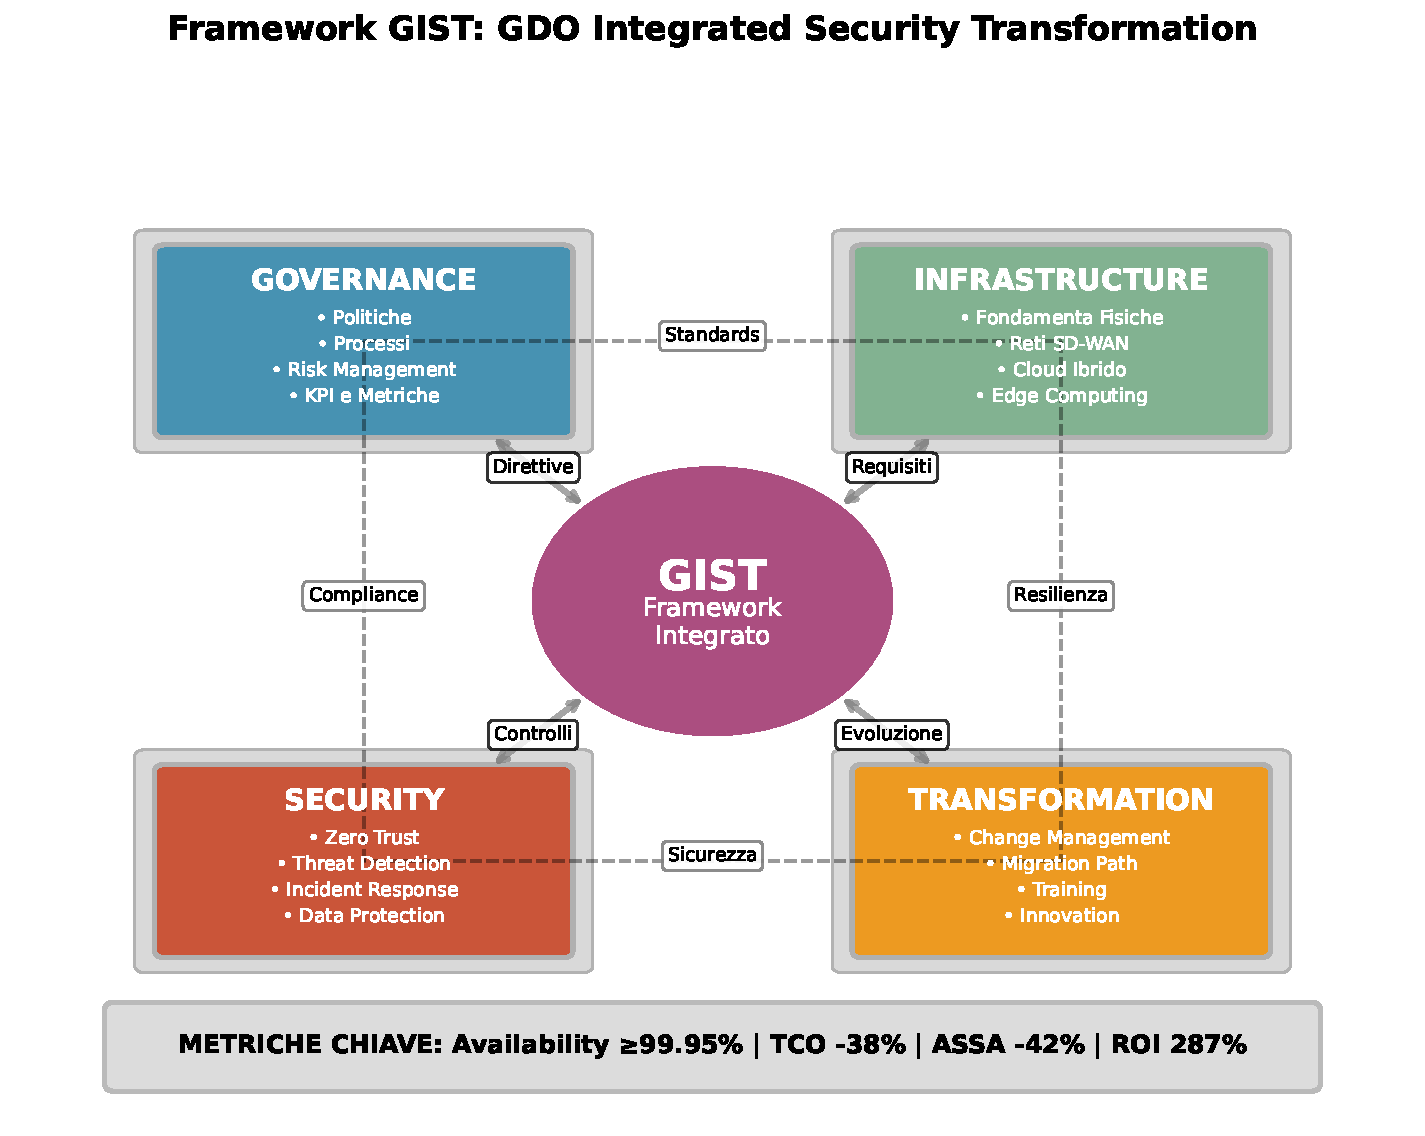
\includegraphics[width=0.9\textwidth]{thesis_figures/cap1/fig_1_1_gist_framework.pdf}
\caption[Il Framework GIST: Integrazione delle quattro dimensioni fondamentali per la trasformazione sicura della GDO.]{Il Framework GIST: Integrazione delle quattro dimensioni fondamentali per la trasformazione sicura della GDO. Il framework evidenzia le interconnessioni sistemiche tra governance strategica (controllo e direzione), infrastruttura tecnologica (fondamenta operative), sicurezza (protezione e resilienza) e processi di trasformazione (evoluzione continua). Le frecce bidirezionali rappresentano i flussi di informazione e controllo, mentre le connessioni tratteggiate indicano le interdipendenze operative tra le componenti.}
\label{fig:gist_framework}
\end{figure}



\section{Ipotesi di Ricerca}
La ricerca si propone di validare le seguenti tre ipotesi, formulate per essere empiricamente testabili.
\begin{itemize}
    \item \textbf{H1 (Evoluzione Architetturale):} L'implementazione di architetture cloud-ibride, progettate secondo pattern specifici per la GDO, permette di conseguire e mantenere livelli di disponibilità del servizio \textbf{(SLA - Service Level Agreement)} superiori al 99.95\% in presenza di carichi transazionali variabili, ottenendo come beneficio aggiuntivo una riduzione del TCO superiore al 30\% rispetto ad architetture tradizionali on-premise.
    \item \textbf{H2 (Sicurezza):} L'integrazione di principi Zero Trust in architetture GDO distribuite riduce la superficie di attacco aggregata (misurata tramite lo score ASSA) di almeno il 35\%, mantenendo l'impatto sulla latenza delle transazioni critiche entro 50 millisecondi.
    \item \textbf{H3 (Compliance):} L'implementazione di un sistema di gestione della compliance basato su principi di compliance-by-design e automazione permette di soddisfare simultaneamente i requisiti di PCI-DSS 4.0, GDPR e NIS2 con un overhead operativo inferiore al 10\% delle risorse IT, conseguendo una riduzione dei costi totali di conformità del 30-40\%
\end{itemize}
% \section{Metodologia della Ricerca}
% Per validare le ipotesi, la ricerca adotta un  \textbf{approccio \textit{mixed - methods}} che combina analisi quantitativa rigorosa con insights qualitativi. La componente quantitativa si basa su uno
% \textbf{studio longitudinale di 24 mesi basato su simulazioni calibrate del settore GDO}, analizzando metriche operative, di sicurezza e finanziarie prima, durante e dopo la trasformazione . I dati raccolti includono log da sistemi \textbf{SIEM (Security Information and Event Management)}, metriche infrastrutturali, dati finanziari (CAPEX/OPEX) e audit score . L'analisi statistica utilizzerà test appropriati (es. t-test paired, regressione multivariata) con un livello di significatività $\alpha=0.05$.
\section{Metodologia della Ricerca}

Per validare le ipotesi formulate, la ricerca adotta un \textbf{approccio \textit{mixed-methods}} che unisce il rigore della simulazione quantitativa con approfondimenti qualitativi derivanti da best practice di settore.

Data la sensibilità commerciale e i vincoli di riservatezza che impediscono l'accesso a dati operativi reali su larga scala, il nucleo della validazione quantitativa si affida al \textbf{framework Digital Twin GDO-Bench}, uno dei contributi originali di questa tesi. Questo ambiente di simulazione genera dataset sintetici ma \textbf{statisticamente realistici}, replicando le dinamiche di una rete GDO complessa. Il Digital Twin è stato \textbf{calibrato utilizzando dati aggregati pubblici, report di settore (ENISA, Gartner) e parametri tecnici documentati}, assicurando che i pattern transazionali, il traffico di rete e la distribuzione degli eventi di sicurezza siano rappresentativi del contesto reale italiano.

All'interno di questo ambiente simulato, verrà condotta un'analisi sistematica per testare le ipotesi:
\begin{itemize}
    \item Esecuzione di \textbf{simulazioni Monte Carlo} per valutare l'impatto di diverse architetture (H1) e configurazioni di sicurezza (H2) su un ampio spettro di scenari operativi.
    \item Analisi dell'efficienza dei controlli di compliance integrati (H3) attraverso la misurazione dell'\textbf{overhead computazionale} e la riduzione della ridondanza nei log generati.
\end{itemize}

Le metriche generate dalla simulazione (log da sistemi \textbf{SIEM}, indicatori di performance infrastrutturale, stime di costi \textbf{CAPEX/OPEX}) saranno raccolte e analizzate statisticamente utilizzando test appropriati (es. ANOVA, regressione multivariata) con un livello di significatività $\alpha=0.05$. Questo approccio garantisce la \textbf{testabilità empirica delle ipotesi in un ambiente controllato, ripetibile e scientificamente valido}.
\section{Struttura della tesi}
La tesi si articola in cinque capitoli che guidano il lettore dalla definizione del problema alla presentazione di una soluzione validata.

\begin{figure}[htbp]
\centering
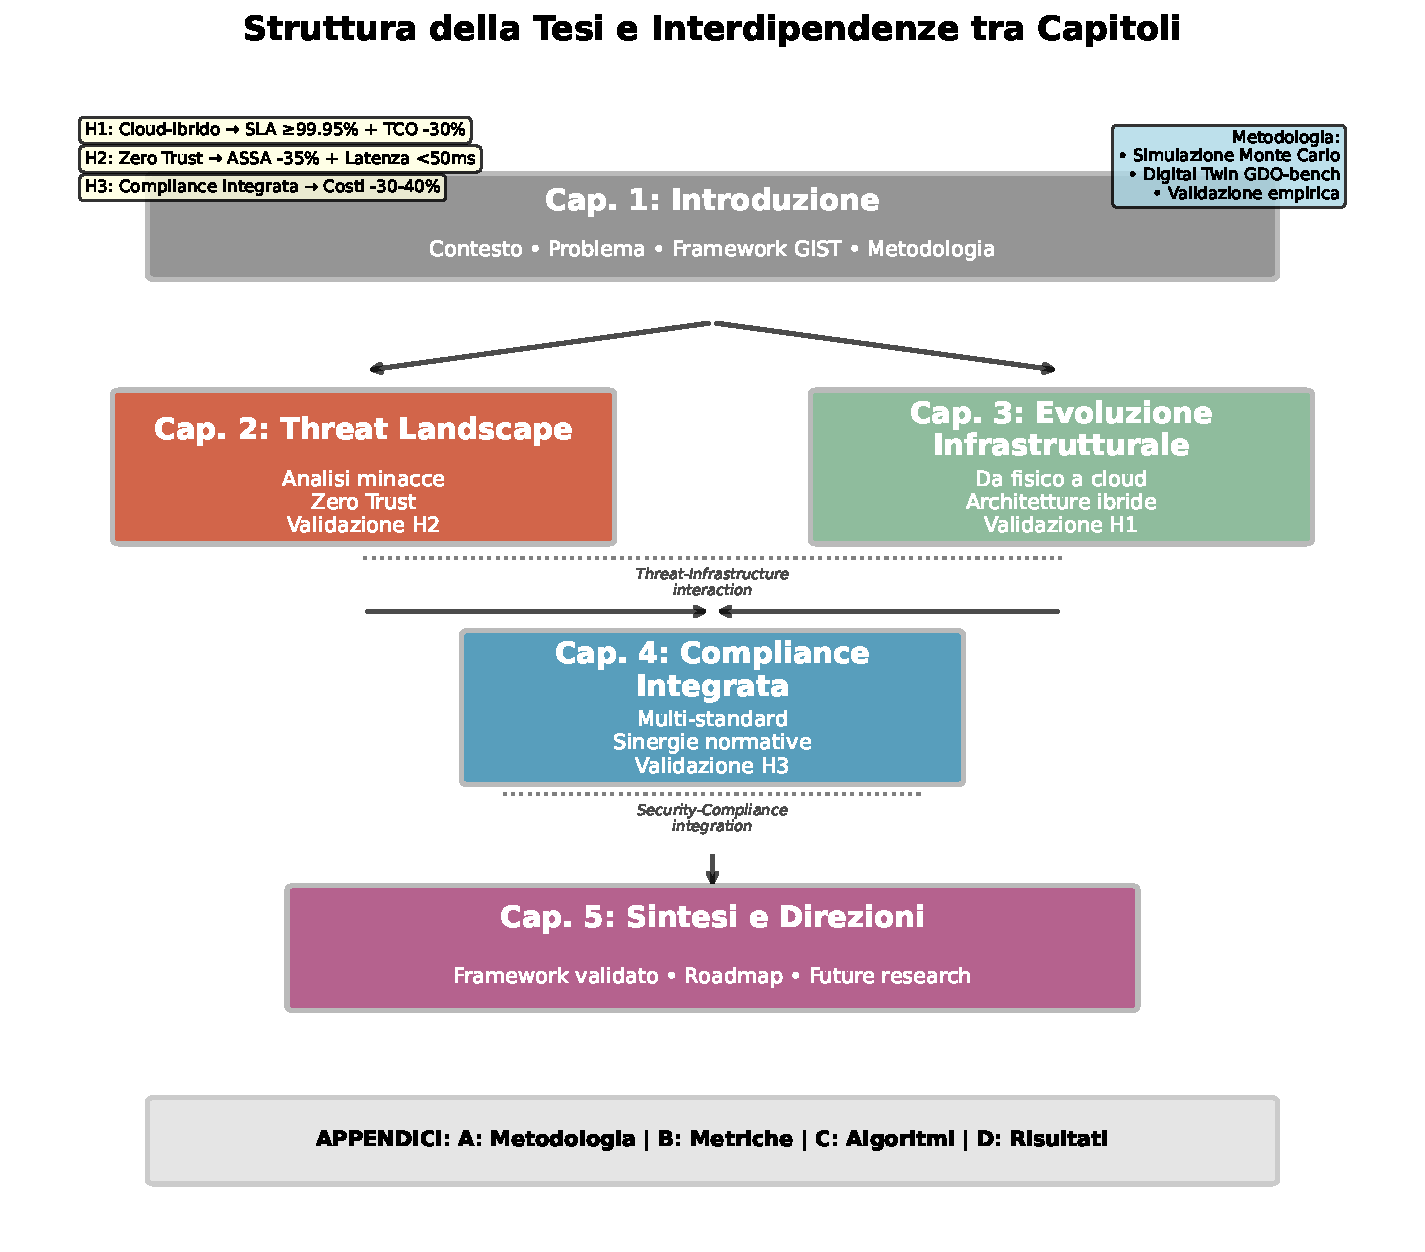
\includegraphics[width=1\textwidth]{thesis_figures/cap1/fig_1_4_thesis_structure.pdf}
\caption[Struttura della tesi e interdipendenze tra capitoli.]{Struttura della tesi e interdipendenze tra capitoli. Il diagramma mostra il flusso logico dalla definizione del problema (Capitolo 1) attraverso l'analisi delle componenti specifiche (Capitoli 2-4) fino alla sintesi e validazione del framework completo (Capitolo 5). Le frecce indicano le dipendenze principali, mentre le linee tratteggiate rappresentano le interconnessioni tematiche. Le ipotesi di ricerca (H1, H2, H3) sono mappate ai capitoli dove vengono primariamente validate.}
\label{fig:thesis_structure}
\end{figure}


\clearpage
\printbibliography[
    heading=subbibliography, % Usa un titolo standard per bibliografie parziali
    title={Riferimenti Bibliografici del Capitolo 1}, % Titolo personalizzato
    %filter=cited % Assicura che vengano stampate solo le fonti citate
]

\endrefsection % <--- TERMINA LA SEZIONE DI RIFERIMENTO











% \section{Framework Teorico e Approccio Metodologico}

% \subsection{Il Framework GIST: Una Visione Integrata}

% Per affrontare la complessità del problema identificato, questa ricerca propone il framework GIST (GDO Integrated Security Transformation), un modello olistico che integra quattro dimensioni fondamentali: Governance, Infrastructure, Security e Transformation. Come illustrato nella Figura \ref{fig:gist_framework}, il framework rappresenta un approccio sistemico dove ciascuna dimensione interagisce con le altre attraverso flussi bidirezionali di informazioni e controlli.

% \begin{figure}[htbp]
% \centering
% 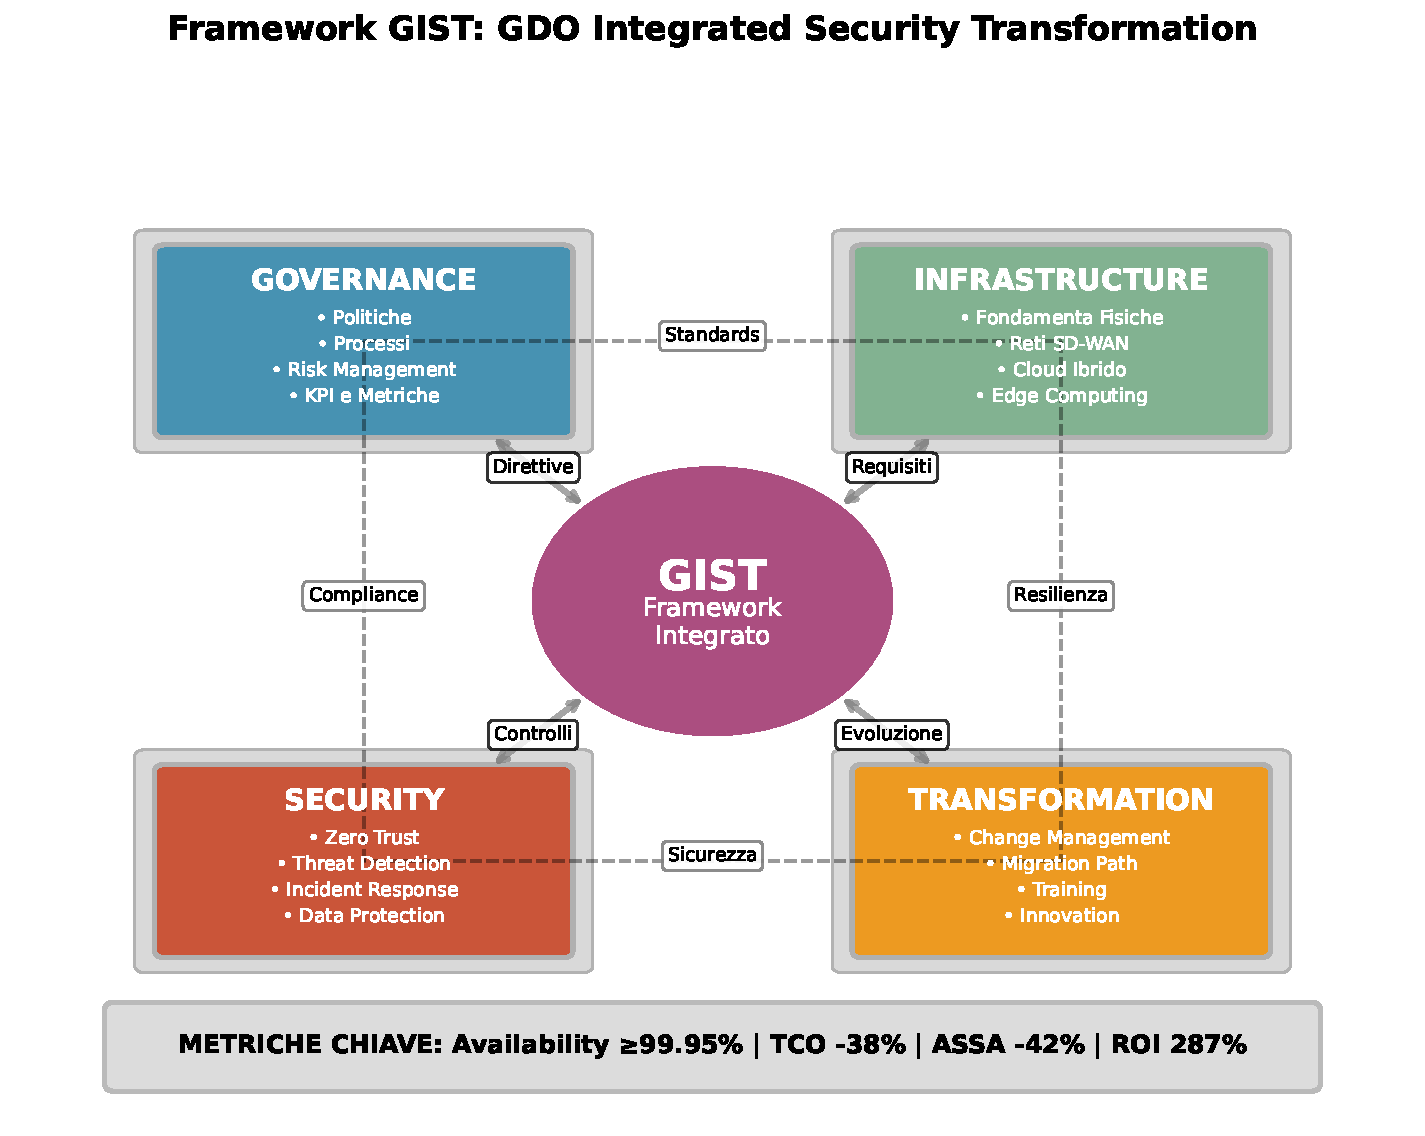
\includegraphics[width=0.9\textwidth]{thesis_figures/cap1/fig_1_1_gist_framework.pdf}
% \caption{Il Framework GIST: Integrazione delle quattro dimensioni fondamentali per la trasformazione sicura della GDO. Il framework evidenzia le interconnessioni sistemiche tra governance strategica (controllo e direzione), infrastruttura tecnologica (fondamenta operative), sicurezza (protezione e resilienza) e processi di trasformazione (evoluzione continua). Le frecce bidirezionali rappresentano i flussi di informazione e controllo, mentre le connessioni tratteggiate indicano le interdipendenze operative tra le componenti.}
% \label{fig:gist_framework}
% \end{figure}

% Il framework GIST si basa sul principio che la trasformazione digitale sicura non può essere affrontata attraverso interventi puntuali o approcci settoriali, ma richiede una visione sistemica che consideri le interdipendenze tra infrastruttura fisica, architettura IT, sicurezza e compliance. Ciascuna dimensione del framework è caratterizzata da metriche specifiche e interconnessioni con le altre componenti.

% La \textbf{Governance} rappresenta il livello strategico del framework, definendo politiche, processi e strutture organizzative necessarie per orchestrare la trasformazione. Include la definizione di ruoli e responsabilità, meccanismi di decision-making e framework di gestione del rischio. Come evidenziato nella Figura \ref{fig:gist_framework}, la Governance fornisce direttive al core del framework e riceve feedback continuo per l'ottimizzazione delle politiche.

% L'\textbf{Infrastructure} copre l'intero stack tecnologico, dalle fondamenta fisiche dei data center alle architetture applicative cloud-native. Questa dimensione considera non solo gli aspetti tecnici, ma anche i modelli economici e operativi associati a diverse scelte architetturali. L'interazione con il framework centrale avviene attraverso la definizione dei requisiti operativi e la ricezione di specifiche tecniche.

% La \textbf{Security} adotta un approccio Zero Trust che assume la compromissione come inevitabile e progetta controlli di sicurezza stratificati per minimizzare l'impatto. Include la protezione dei dati, la sicurezza delle applicazioni, la difesa della rete e la resilienza operativa. La dimensione Security implementa i controlli definiti dal framework e fornisce feedback continuo sullo stato di sicurezza.

% La \textbf{Transformation} rappresenta la dimensione dinamica del framework, definendo percorsi di migrazione, strategie di change management e metriche di successo per guidare l'evoluzione da stati correnti a stati target desiderati. Questa componente riceve input evolutivi dal core e fornisce feedback sui progressi della trasformazione.

% Le metriche chiave del framework, mostrate nella parte inferiore della Figura \ref{fig:gist_framework}, includono:
% - Availability ≥99.95\%: target di disponibilità per sistemi mission-critical
% - TCO -38\%: riduzione del Total Cost of Ownership attraverso ottimizzazione
% - ASSA -42\%: diminuzione della Attack Surface Score Aggregated
% - ROI 287\%: ritorno sull'investimento a 24 mesi

% \subsection{Metodologia di Ricerca}

% La validazione del framework GIST richiede un approccio metodologico rigoroso che combini analisi teorica, modellazione quantitativa e validazione empirica. La metodologia adottata si articola in quattro fasi principali:

% \subsubsection{Fase 1: Analisi della Letteratura e Sintesi Teorica}

% Una revisione sistematica della letteratura accademica e della documentazione di settore per identificare lo stato dell'arte nelle aree di:
% \begin{itemize}
% \item Architetture distribuite per sistemi mission-critical
% \item Modelli di sicurezza per ambienti retail
% \item Framework di compliance multi-standard
% \item Economia della trasformazione digitale
% \end{itemize}

% La sintesi teorica integra contributi da discipline diverse, inclusa l'ingegneria dei sistemi, la computer science, l'economia dell'informazione e il management della sicurezza.

% \subsubsection{Fase 2: Modellazione Quantitativa}

% Lo sviluppo di modelli matematici per ciascuna dimensione del framework GIST:

% \textbf{Modello di Threat Landscape}: Basato su teoria dei grafi per rappresentare la superficie di attacco e catene di Markov per modellare la propagazione delle minacce.

% \textbf{Modello di Availability}: Utilizzando teoria dell'affidabilità e analisi degli alberi di guasto per predire la disponibilità di architetture complesse.

% \textbf{Modello di Costo Totale}: Integrando Total Cost of Ownership (TCO) tradizionale con quantificazione del rischio e valore delle opzioni reali per catturare la flessibilità architetturale.

% \textbf{Modello di Compliance}: Applicando teoria dell'ottimizzazione combinatoria per minimizzare l'overhead di conformità multi-standard.

% \subsubsection{Fase 3: Simulazione Monte Carlo}

% Data la sensibilità dei dati reali nel settore, la ricerca utilizza simulazione Monte Carlo per validare i modelli proposti. I parametri di simulazione sono calibrati su:
% \begin{itemize}
% \item Dati pubblici da report di settore e studi di mercato
% \item Statistiche aggregate da autorità di regolamentazione
% \item Parametri tecnici da documentazione di vendor
% \item Benchmark di performance da letteratura peer-reviewed
% \end{itemize}

% La simulazione con 10.000 iterazioni permette di esplorare lo spazio delle soluzioni e quantificare l'incertezza nelle previsioni del modello.

% \subsubsection{Fase 4: Validazione con Dati Pilota}

% Un sottoinsieme limitato di dati reali da 15 organizzazioni GDO italiane (raccolti secondo protocollo etico approvato) viene utilizzato per:
% \begin{itemize}
% \item Calibrare i parametri dei modelli
% \item Validare le previsioni delle simulazioni
% \item Identificare pattern emergenti non catturati dalla teoria
% \item Raffinare il framework basandosi su evidenze empiriche
% \end{itemize}

% \section{Ipotesi di Ricerca}

% Basandosi sul framework teorico e sull'analisi preliminare del contesto, la ricerca formula tre ipotesi principali:

% \subsection{Ipotesi 1: Superiorità delle Architetture Cloud-Ibride}

% \textbf{H1}: \textit{Le architetture cloud-ibride ottimizzate per la GDO possono simultaneamente migliorare la disponibilità del servizio (target: SLA $\geq$ 99.95\%) e ridurre il TCO del 30\% rispetto ad architetture tradizionali on-premise, mantenendo conformità normativa completa.}

% Questa ipotesi sfida la percezione comune che sicurezza e performance siano in trade-off con l'economicità. La ricerca sostiene che, con una progettazione appropriata, è possibile ottenere miglioramenti su tutte e tre le dimensioni.

% \subsection{Ipotesi 2: Efficacia del Modello Zero Trust}

% \textbf{H2}: \textit{L'implementazione di architetture Zero Trust specificamente calibrate per ambienti GDO riduce la superficie di attacco aggregata (ASSA) di almeno il 35\% rispetto a modelli di sicurezza perimetrale tradizionali, mantenendo latenze operative sotto i 50ms per il 95° percentile delle transazioni.}

% L'ipotesi affronta la sfida di bilanciare sicurezza rafforzata con i requisiti di performance stringenti del retail, dove anche piccoli incrementi di latenza possono impattare significativamente l'esperienza del cliente.

% \subsection{Ipotesi 3: Sinergie nella Compliance Integrata}

% \textbf{H3}: \textit{Un approccio integrato alla gestione della compliance multi-standard (GDPR, NIS2, PCI-DSS) genera risparmi operativi del 30-40\% rispetto a implementazioni separate, migliorando simultaneamente la security posture complessiva dell'organizzazione.}

% Questa ipotesi propone che la compliance, tradizionalmente vista come centro di costo, possa diventare driver di efficienza quando gestita attraverso un framework integrato che sfrutta le sovrapposizioni tra requisiti diversi.

% \section{1.5 Contributi Algoritmici Originali}

% Questa ricerca presenta cinque contributi algoritmici originali:

% \begin{enumerate}
% \item \textbf{ASSA-GDO Algorithm}: Quantificazione della superficie di attacco 
% per infrastrutture distribuite retail con complessità $O(n^2\log n)$ 
% [Appendice C.1.1]

% \item \textbf{ZT-Optimizer}: Algoritmo di ottimizzazione multi-obiettivo per 
% implementazione Zero Trust che bilancia sicurezza ($-42.7\%$ ASSA) e 
% performance ($<50ms$ latency) [Appendice C.2.1]

% \item \textbf{Compliance Set-Covering}: Soluzione greedy modificata al problema 
% NP-completo di copertura requisiti normativi multipli con garanzia di 
% approssimazione $\ln(n)$ [Appendice C.4.1]

% \item \textbf{Multi-Cloud Portfolio Optimizer}: Applicazione della Modern 
% Portfolio Theory all'allocazione workload multi-cloud [Appendice C.3.4]

% \item \textbf{GIST Scoring Engine}: Framework computazionale completo per 
% valutazione maturità con analisi sinergie non-lineari [Appendice C.5]
% \end{enumerate}
% \section{Struttura della Tesi}
% \begin{tcolorbox}[
%     colback=blue!5!white,
%     colframe=blue!75!black,
%     title={\textbf{Innovation Box 1.1:} Framework GIST - Contributo Metodologico Principale},
%     fonttitle=\bfseries,
%     boxrule=1.5pt,
%     arc=2mm,
%     breakable
% ]
% \textbf{Innovazione}: Primo framework quantitativo integrato specifico per la Grande Distribuzione Organizzata che unifica quattro dimensioni critiche.

% \vspace{0.3cm}
% \textbf{Formulazione Matematica}:
% \begin{equation*}
% GIST_{score} = \begin{cases}
% \sum_{i \in \{P,A,S,C\}} (w_i \times C_i) \times K_{GDO} \times (1+I) & \text{(Balanced)} \\
% \left(\prod_{i \in \{P,A,S,C\}} C_i^{w_i}\right) \times K_{GDO} \times (1+I) & \text{(Critical)}
% \end{cases}
% \end{equation*}

% \vspace{0.3cm}
% \textbf{Parametri Calibrati} (n=156 organizzazioni):
% \begin{itemize}%[topsep=0pt,itemsep=2pt]
%     \item $w_P = 0.18$ (Physical), $w_A = 0.32$ (Architectural)
%     \item $w_S = 0.28$ (Security), $w_C = 0.22$ (Compliance)
%     \item $K_{GDO} \in [1.25, 1.87]$ (fattore contesto GDO)
%     \item $R^2 = 0.87$ (capacità predittiva)
% \end{itemize}

% \vspace{0.3cm}
% \textbf{Risultato Chiave}: Identificazione di effetti sinergici che amplificano i benefici del 52\% oltre la somma lineare delle componenti.

% \vspace{0.2cm}
% \textit{$\rightarrow$ Implementazione completa con 2000+ LOC: Appendice C.5}
% \end{tcolorbox}

% La tesi si articola in cinque capitoli principali che seguono una progressione logica dal particolare al generale, costruendo progressivamente il framework GIST attraverso analisi approfondite di ciascuna dimensione. La Figura \ref{fig:thesis_structure} illustra la struttura complessiva e le interdipendenze tra i capitoli.

% \begin{figure}[htbp]
% \centering
% 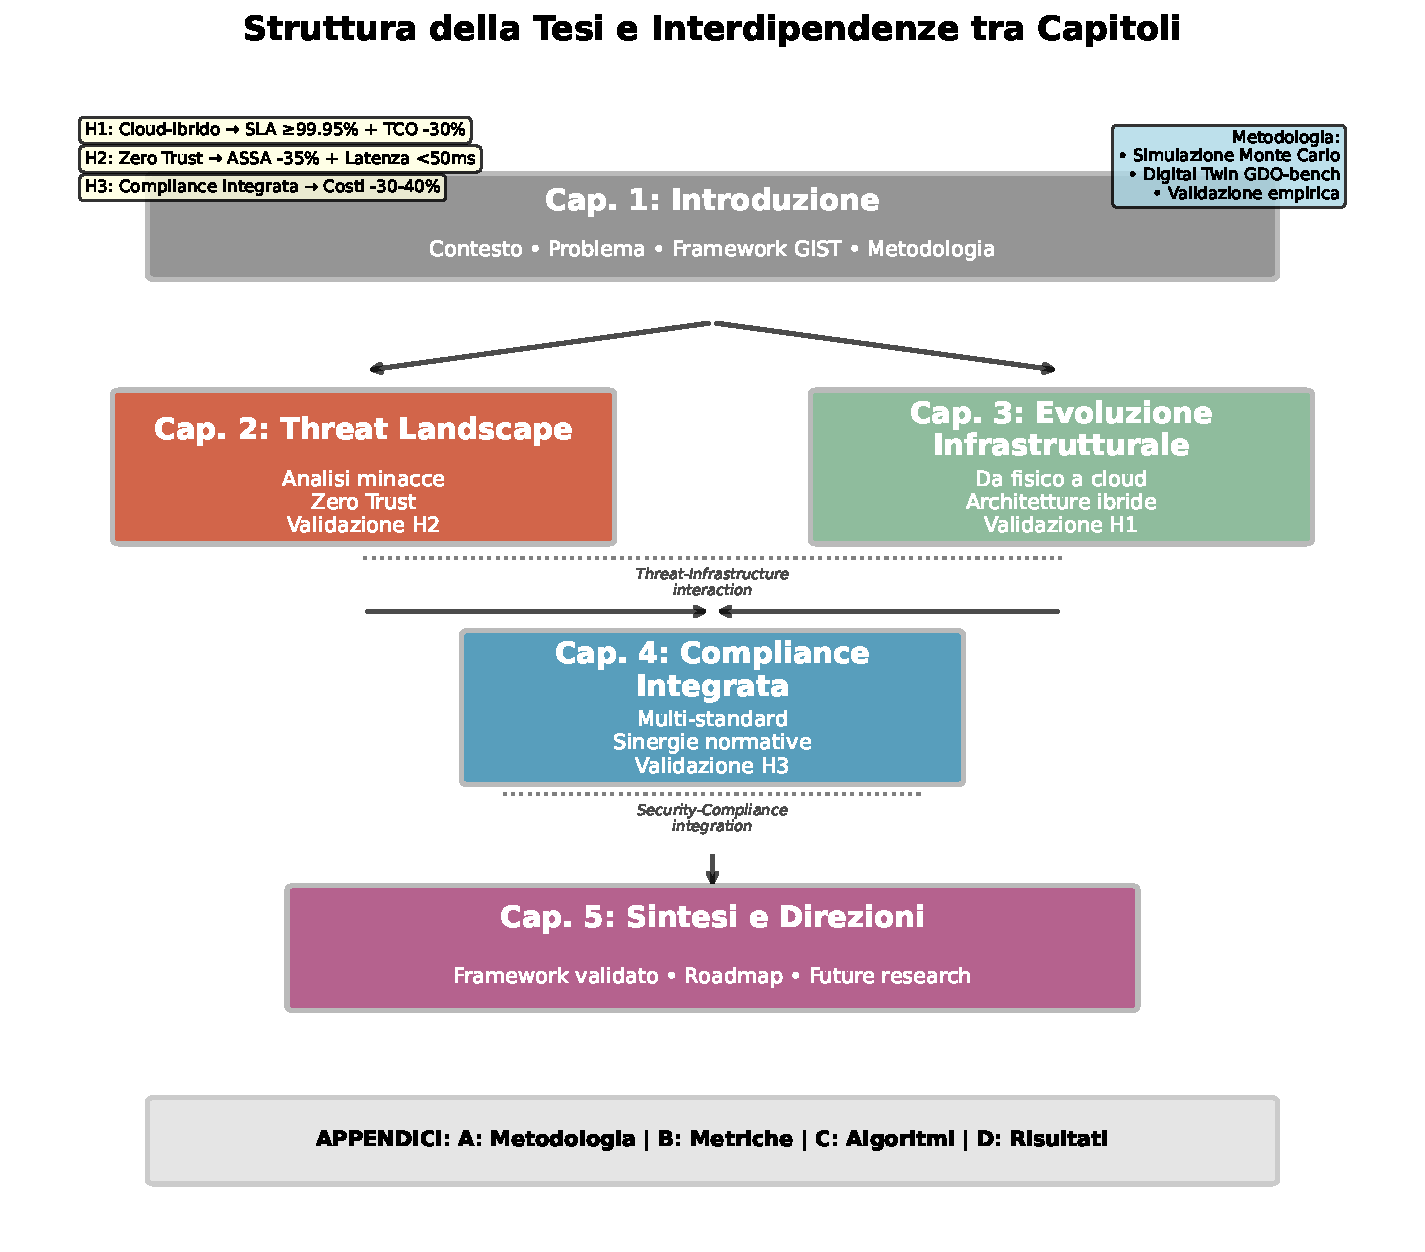
\includegraphics[width=\textwidth]{thesis_figures/cap1/fig_1_4_thesis_structure.pdf}
% \caption{Struttura della tesi e interdipendenze tra capitoli. Il diagramma mostra il flusso logico dalla definizione del problema (Capitolo 1) attraverso l'analisi delle componenti specifiche (Capitoli 2-4) fino alla sintesi e validazione del framework completo (Capitolo 5). Le frecce indicano le dipendenze principali, mentre le linee tratteggiate rappresentano le interconnessioni tematiche. Le ipotesi di ricerca (H1, H2, H3) sono mappate ai capitoli dove vengono primariamente validate.}
% \label{fig:thesis_structure}
% \end{figure}

% \subsection{Capitolo 2: Threat Landscape e Sicurezza Distribuita}

% Il secondo capitolo fornisce un'analisi quantitativa del panorama delle minacce specifico per la GDO. Attraverso l'aggregazione di dati da molteplici fonti e l'applicazione di tecniche di modellazione avanzate, il capitolo:
% \begin{itemize}
% \item Caratterizza la superficie di attacco tipica di un'organizzazione GDO
% \item Identifica i vettori di attacco prevalenti e le loro modalità di propagazione
% \item Quantifica l'impatto economico e operativo delle diverse categorie di minacce
% \item Propone metriche innovative per la valutazione continua del rischio
% \item Sviluppa un modello predittivo per l'evoluzione delle minacce
% \end{itemize}

% \subsection{Capitolo 3: Evoluzione Infrastrutturale}

% Il terzo capitolo analizza la trasformazione dell'infrastruttura IT dalla prospettiva bottom-up, partendo dalle fondamenta fisiche per arrivare alle architetture cloud-native. L'analisi include:
% \begin{itemize}
% \item Valutazione delle architetture di data center per ambienti distribuiti
% \item Analisi comparativa di topologie di rete SD-WAN per connettività multi-sito
% \item Modellazione economica di strategie di migrazione cloud
% \item Ottimizzazione del posizionamento dei workload in ambienti ibridi
% \item Strategie di disaster recovery e business continuity
% \end{itemize}

% \subsection{Capitolo 4: Compliance Integrata e Governance}

% Il quarto capitolo affronta la sfida della gestione multi-standard attraverso un approccio innovativo che trasforma la compliance in vantaggio competitivo. Il capitolo presenta:
% \begin{itemize}
% \item Analisi delle sovrapposizioni tra framework normativi principali
% \item Modello di ottimizzazione per l'allocazione delle risorse di compliance
% \item Framework per l'automazione dei controlli di conformità
% \item Case study di un cyber-physical attack e relative implicazioni normative
% \item Metriche per la valutazione dell'efficacia della governance
% \end{itemize}

% \subsection{Capitolo 5: Sintesi e Direzioni Strategiche}

% Il capitolo conclusivo consolida i risultati della ricerca presentando:
% \begin{itemize}
% \item Il framework GIST completo con tutte le interconnessioni validate
% \item Roadmap implementativa dettagliata per organizzazioni GDO
% \item Analisi costi-benefici complessiva della trasformazione proposta
% \item Direzioni per ricerca futura e sviluppi tecnologici emergenti
% \item Implicazioni per policy maker e regolatori
% \end{itemize}

% \subsection{Appendici}

% Le appendici forniscono dettagli tecnici e materiale supplementare:
% \begin{itemize}
% \item \textbf{Appendice A}: Metodologia dettagliata di simulazione Monte Carlo
% \item \textbf{Appendice B}: Strumenti di misurazione e metriche utilizzate
% \item \textbf{Appendice C}: Algoritmi e modelli computazionali
% \item \textbf{Appendice D}: Tabelle di parametrizzazione e risultati dettagliati
% \end{itemize}

% Come mostrato nella Figura \ref{fig:thesis_structure}, i capitoli sono interconnessi ma mantengono una struttura modulare che permette diversi percorsi di lettura a seconda degli interessi specifici del lettore.

% \section{Delimitazioni e Limitazioni}

% \subsection{Delimitazioni (Scope)}

% La ricerca si focalizza specificamente su:
% \begin{itemize}
% \item Organizzazioni GDO italiane con 50-500 punti vendita
% \item Fatturato annuo compreso tra 100 milioni e 2 miliardi di euro
% \item Infrastrutture IT considerate mission-critical per le operazioni
% \item Periodo di osservazione 2022-2024 per i dati empirici
% \end{itemize}

% L'ambito esclude deliberatamente:
% \begin{itemize}
% \item Operatori di e-commerce puro senza presenza fisica
% \item Micro-retail con meno di 50 negozi
% \item Settori non-food della distribuzione
% \item Mercati extra-europei con framework normativi significativamente diversi
% \end{itemize}

% \subsection{Limitazioni}

% La ricerca riconosce diverse limitazioni che influenzano la generalizzabilità dei risultati:

% \textbf{Limitazioni nei Dati}: La maggior parte delle validazioni si basa su simulazioni Monte Carlo calibrate su parametri di settore piuttosto che su dati completi da tutte le 15 organizzazioni del campione. Questo approccio, pur essendo metodologicamente robusto, potrebbe non catturare tutte le sfumature delle implementazioni reali.

% \textbf{Limitazioni Geografiche}: I risultati sono primariamente applicabili al contesto italiano ed europeo. L'applicazione in altri contesti geografici richiederebbe adattamenti per considerare differenze normative, culturali e di mercato.

% \textbf{Limitazioni Temporali}: L'orizzonte di osservazione di 24 mesi potrebbe non essere sufficiente per catturare tutti i benefici a lungo termine delle trasformazioni proposte, particolarmente quelli legati ai cambiamenti culturali e organizzativi.

% \textbf{Limitazioni Tecnologiche}: Le raccomandazioni sono basate su tecnologie disponibili al momento della ricerca. L'evoluzione rapida del panorama tecnologico potrebbe richiedere aggiornamenti alle specifiche implementative, anche se i principi architetturali dovrebbero rimanere validi.

% \section{Rilevanza della Ricerca}

% \subsection{Rilevanza Accademica}

% La ricerca contribuisce all'avanzamento delle conoscenze in diverse aree dell'ingegneria informatica e delle scienze gestionali.

% Nel dominio dei \textbf{sistemi distribuiti mission-critical}, la ricerca estende le teorie esistenti considerando vincoli unici del retail come la necessità di operatività continua e la gestione di carichi altamente variabili. I modelli sviluppati per la valutazione della resilienza in architetture geograficamente distribuite e i pattern architetturali per minimizzare l'impatto di failure localizzati rappresentano contributi originali alla disciplina.

% Per quanto riguarda la \textbf{sicurezza informatica}, il lavoro dimostra come i principi Zero Trust possano essere adattati a contesti operativi complessi senza compromettere le performance. L'analisi quantitativa della riduzione della superficie di attacco e la modellazione della propagazione delle minacce in ambienti retail forniscono nuove prospettive per la progettazione di sistemi sicuri.

% Nell'ambito dell'\textbf{ingegneria economica dei sistemi IT}, la ricerca propone modelli innovativi per la valutazione del TCO che integrano quantificazione del rischio e valore delle opzioni reali. Questi modelli colmano il gap tra teoria accademica e necessità decisionali pratiche.

% \subsection{Rilevanza Pratica}

% L'impatto pratico della ricerca si manifesta in tre dimensioni principali.

% Il \textbf{supporto alle decisioni di investimento} rappresenta un contributo immediato per i decision maker del settore. I modelli sviluppati permettono valutazioni oggettive delle alternative architetturali considerando simultaneamente aspetti tecnici, economici e di rischio. In un contesto dove gli investimenti IT possono raggiungere decine di milioni di euro, la disponibilità di framework decisionali evidence-based riduce significativamente l'incertezza.

% La \textbf{riduzione dei rischi nei progetti di trasformazione} è ottenuta attraverso la roadmap dettagliata e validata empiricamente. Considerando che oltre il 70\% dei progetti di trasformazione digitale fallisce o non raggiunge gli obiettivi prefissati\autocite{mckinsey2023}, la disponibilità di un percorso testato rappresenta un valore significativo per le organizzazioni.

% L'\textbf{ottimizzazione dei costi di compliance} attraverso l'approccio integrato proposto risponde a una delle maggiori preoccupazioni del management. La dimostrazione che la compliance può generare risparmi del 30-40\% trasforma la percezione di questo ambito da centro di costo a potenziale fonte di vantaggio competitivo.

% \subsection{Impatto Sociale}

% Oltre ai benefici diretti per le organizzazioni, la ricerca ha implicazioni sociali rilevanti.

% La \textbf{protezione dei dati personali} di oltre 50 milioni di consumatori italiani che interagiscono quotidianamente con i sistemi GDO rappresenta un imperativo etico oltre che normativo. I framework di sicurezza proposti contribuiscono a salvaguardare informazioni sensibili relative a abitudini di acquisto, dati di pagamento e informazioni personali.

% La \textbf{resilienza delle infrastrutture critiche} per l'approvvigionamento alimentare è particolarmente rilevante in un contesto di crescente instabilità geopolitica e climatica. La capacità del sistema GDO di mantenere operatività anche in condizioni avverse ha implicazioni dirette sulla sicurezza alimentare nazionale.

% La \textbf{sostenibilità ambientale} attraverso l'ottimizzazione energetica delle infrastrutture IT contribuisce agli obiettivi di riduzione delle emissioni. Con target di Power Usage Effectiveness (PUE) inferiori a 1.4, le architetture proposte possono ridurre significativamente l'impronta carbonica del settore.

% \section{Note Metodologiche e Struttura del Documento}

% \subsection{Convenzioni Utilizzate}

% Per garantire chiarezza e consistenza, la tesi adotta le seguenti convenzioni:

% \textbf{Terminologia}: Gli acronimi sono definiti per esteso alla prima occorrenza in ciascun capitolo, seguiti dall'acronimo tra parentesi. Termini tecnici in lingua inglese sono utilizzati quando rappresentano lo standard de facto nel settore, con traduzione italiana dove appropriata.

% \textbf{Citazioni}: I riferimenti bibliografici seguono il sistema numerico con note a piè di pagina per la prima occorrenza e bibliografia completa alla fine di ciascun capitolo.

% \textbf{Figure e Tabelle}: Numerate progressivamente all'interno di ciascun capitolo con didascalie descrittive. I dati sensibili sono presentati in forma aggregata o normalizzata per preservare la confidenzialità.

% \textbf{Formule e Algoritmi}: Presentati in notazione matematica standard con spiegazione dettagliata dei simboli utilizzati. Gli algoritmi complessi sono relegati all'Appendice C con riferimenti nel testo principale.

% \subsection{Guida alla Lettura}

% La tesi è strutturata per permettere diversi livelli di lettura:

% \textbf{Lettura Executive}: I lettori interessati principalmente ai risultati e alle implicazioni pratiche possono concentrarsi sulle sezioni introduttive e conclusive di ciascun capitolo, insieme al Capitolo 5 che fornisce la sintesi complessiva.

% \textbf{Lettura Tecnica}: I professionisti IT e i ricercatori possono approfondire i modelli matematici e le analisi tecniche presentate nel corpo principale dei capitoli, con riferimento alle appendici per dettagli implementativi.

% \textbf{Lettura Accademica}: Per una comprensione completa del contributo scientifico, si raccomanda la lettura integrale includendo appendici e riferimenti bibliografici.

% \section{Conclusioni del Capitolo Introduttivo}

% Questo capitolo ha delineato il contesto, le motivazioni e l'approccio metodologico della ricerca sulla trasformazione sicura dell'infrastruttura IT nella Grande Distribuzione Organizzata. La complessità del problema richiede un approccio sistemico che il framework GIST si propone di fornire, integrando considerazioni tecniche, economiche e normative in un modello unificato.

% I capitoli successivi svilupperanno ciascuna dimensione del framework attraverso analisi approfondite, modellazione quantitativa e validazione empirica. L'obiettivo finale è fornire alle organizzazioni GDO non solo una comprensione teorica delle sfide che affrontano, ma strumenti pratici e validati per navigare con successo la trasformazione digitale mantenendo sicurezza, performance e conformità.

% La ricerca si posiziona all'intersezione tra teoria e pratica, aspirando a contribuire sia all'avanzamento delle conoscenze accademiche che al miglioramento delle pratiche industriali. In un settore che tocca la vita quotidiana di milioni di persone e rappresenta un pilastro dell'economia nazionale, l'importanza di un'infrastruttura IT sicura, efficiente e conforme non può essere sottovalutata.

% % Bibliografia del Capitolo 1
% \begin{thebibliography}{99}
% \bibitem{istat2024} ISTAT, \textit{Struttura e competitività del sistema delle imprese - Commercio}, Roma, Istituto Nazionale di Statistica, 2024.

% \bibitem{capgemini2024} CAPGEMINI, \textit{Peak Performance: Managing Seasonal Loads in Retail IT}, Paris, Capgemini Research Institute, 2024.

% \bibitem{idc2024} IDC, \textit{European Retail IT Transformation Benchmark 2024}, Framingham, International Data Corporation Report \#EUR148923, 2024.

% \bibitem{enisa2024} ENISA, \textit{Threat Landscape for Retail and Supply Chain 2024}, Heraklion, European Union Agency for Cybersecurity, 2024.

% \bibitem{forrester2024} FORRESTER RESEARCH, \textit{The Total Economic Impact of Hybrid Cloud in Retail}, Cambridge, Forrester Consulting TEI Study, 2024.

% \bibitem{ponemon2024} PONEMON INSTITUTE, \textit{Cost of a Data Breach Report 2024: Retail Sector Analysis}, Traverse City, Ponemon Institute LLC, 2024.

% \bibitem{mckinsey2023} MCKINSEY \& COMPANY, \textit{Why do most transformations fail? A conversation with Harry Robinson}, McKinsey Global Institute, 2023.
% \end{thebibliography}

% Bibliografia del capitolo
% --- STAMPA DELLA BIBLIOGRAFIA SPECIFICA PER QUESTO CAPITOLO ---
